\documentclass[12pt,a4paper]{article}
\usepackage[utf8]{inputenc}
\usepackage{graphicx}
\usepackage{listings}
\usepackage{hyperref}
\usepackage{url}
\usepackage{color}
\usepackage{float}
\usepackage{enumitem}
\usepackage{minted}

\title{E-Commerce System Implementation\\
       Using Python and Flask}
\author{Afolabi Oguntuase}
\date{\today}

\begin{document}

\maketitle
\newpage

\tableofcontents
\newpage

\section{Executive Summary}
This project implements a flexible e-commerce system using Python and Flask, featuring a robust order processing system that handles different types of products and order workflows. The system demonstrates the practical application of object-oriented design patterns and principles.

\section{Project Overview and Objectives}

\subsection{Project Overview}
This project implements an e-commerce system using Python and Flask framework, focusing on order processing and product management. The system is built as a RESTful API that showcases object-oriented programming principles through the implementation of various design patterns.

The system's core functionality includes:

\begin{itemize}
    \item \textbf{Product Management}
    \begin{itemize}
        \item Support for both physical and digital products
        \item Stock tracking for physical products
        \item Product creation and modification by administrators
    \end{itemize}

    \item \textbf{Order Processing}
    \begin{itemize}
        \item Shopping cart functionality
        \item Purchase order processing
        \item Return and exchange handling
    \end{itemize}

    \item \textbf{User Management}
    \begin{itemize}
        \item Role-based access (Admin/Customer)
        \item JWT-based authentication
        \item Secure password handling
    \end{itemize}
\end{itemize}

\subsection{Primary Objectives}

The main objectives of this project are to:

\begin{enumerate}
    \item Demonstrate practical application of OOP principles and design patterns
    \item Implement a flexible and extensible order processing system
    \item Create a secure and scalable user authentication system
    \item Develop a maintainable and well-tested codebase
\end{enumerate}

The system architecture emphasizes:
\begin{itemize}
    \item Modular design through factory patterns
    \item Code reusability through inheritance
    \item Data integrity through proper database relationships using Supabase
    \item Security through role-based access control
\end{itemize}
\section{Design Patterns Implementation}
The following diagrams illustrate the key design patterns used in this project and how they interact:

\begin{figure}[H]
    \centering
    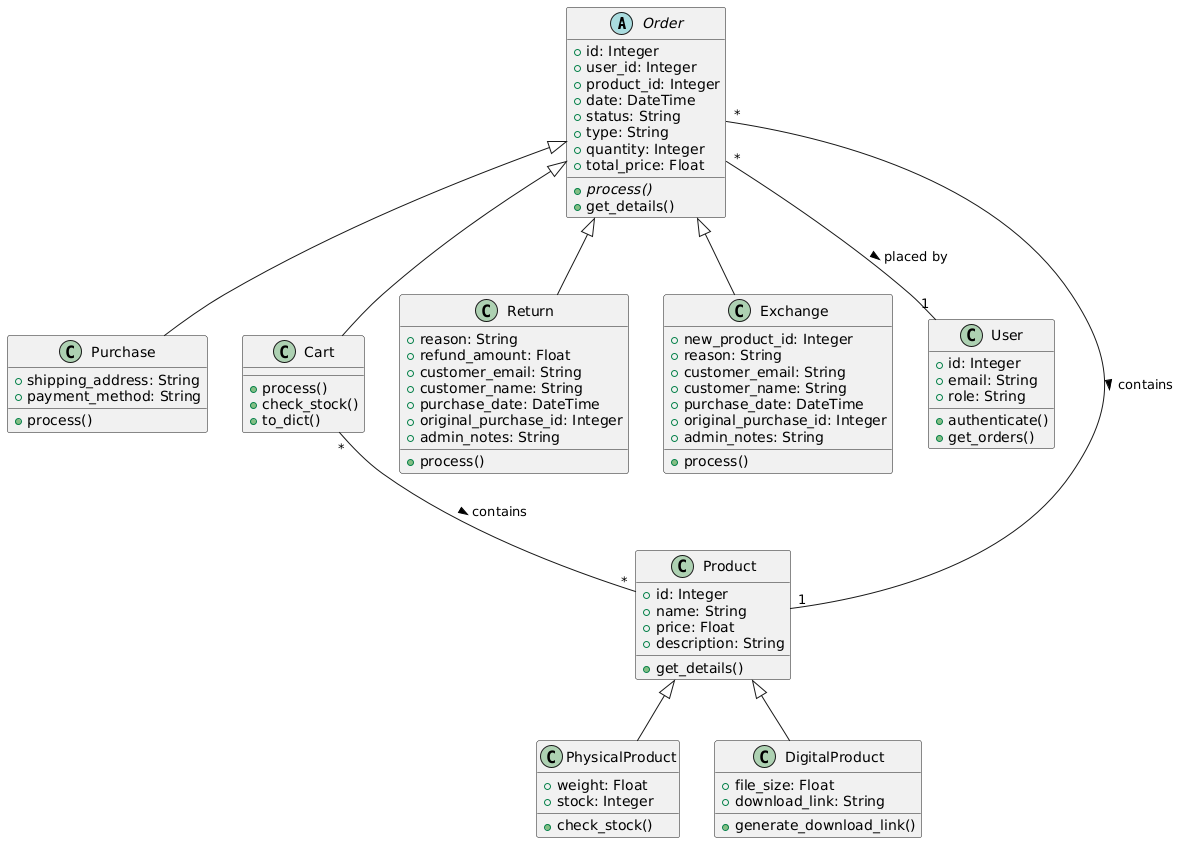
\includegraphics[width=0.8\textwidth]{docs/diagrams/class_diagram.png}
    \caption{Class Diagram Showing Design Patterns}
\end{figure}

The class diagram demonstrates the inheritance hierarchies and relationships between components:
\begin{itemize}
    \item The abstract Order class serves as the base for specialized order types (Purchase, Cart, Return, Exchange)
    \item Products follow a similar hierarchy with PhysicalProduct and DigitalProduct inheriting from Product
    \item Many-to-one relationships exist between Orders and Users ("placed by")
    \item Many-to-many relationships between Cart and Products enable shopping cart functionality
\end{itemize}

\begin{figure}[H]
    \centering
    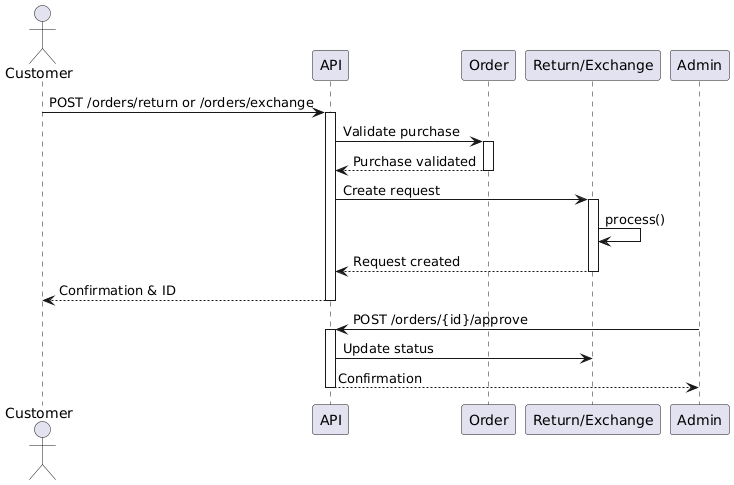
\includegraphics[width=0.8\textwidth]{docs/diagrams/sequence_diagram.png}
    \caption{Sequence Diagram of Pattern Interactions}
\end{figure}

The sequence diagram shows the interaction flow for return/exchange processing:
\begin{itemize}
    \item Customer initiates request through API endpoint
    \item System validates original purchase order
    \item Return/Exchange object is created and processed
    \item Admin reviews and approves/rejects request
\end{itemize}

\begin{figure}[H]
    \centering
    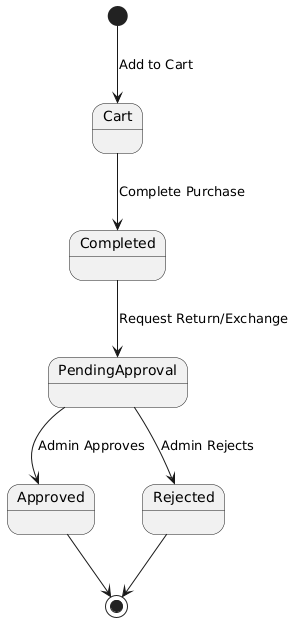
\includegraphics[width=0.8\textwidth]{docs/diagrams/state_diagram.png}
    \caption{State Diagram Showing Order Processing States}
\end{figure}

The state diagram illustrates the lifecycle of an order:
\begin{itemize}
    \item Orders begin in Cart state when items are added
    \item Successful purchase moves order to Completed state
    \item Return/Exchange requests transition to PendingApproval
    \item Admin action results in final Approved or Rejected state
\end{itemize}
\subsection{Creational Patterns}

\subsubsection{Factory Method Pattern}
The project implements the Factory Method pattern in multiple components, most notably in the creation of users, products, and orders. This pattern was chosen to:

\begin{itemize}
    \item Encapsulate object creation logic
    \item Support different types of objects without modifying existing code
    \item Maintain single responsibility principle
\end{itemize}

\paragraph{OrderFactory Implementation}
The OrderFactory (orders/factory.py) demonstrates a clear implementation:
\begin{minted}{python}
class OrderFactory:
    @staticmethod
    def create_order(order_type: str, **kwargs) -> Order:
        match order_type:
            case "purchase":
                return Purchase(**kwargs)
            case "return": 
                return Return(**kwargs)
            case "exchange":
                return Exchange(**kwargs)
            case _:
                raise ValueError(f"Unknown order type: {order_type}")
\end{minted}

This implementation allows:
\begin{itemize}
    \item Dynamic creation of different order types
    \item Easy extension for new order types
    \item Centralized object creation logic
\end{itemize}

\paragraph{Product Factory Usage}
The product creation endpoint (main.py) shows practical application:
# CREATE - Create products
\begin{minted}{python}
@app.route('/products', methods=['POST'])
@admin_required
def create_product(current_user):
    data = request.get_json()
    if isinstance(data, dict):
        data = [data]
    
    created_products = []
    errors = []

    try:
        for product_data in data:
            try:
          
                base_attrs = {
                    'name': product_data['name'],
                    'description': product_data.get('description', ''),
                    'price': product_data['price']
                }

                if product_data['product_type'] == 'physical':
                    base_attrs.update({
                        'weight': product_data.get('weight'),
                        'stock': product_data.get('stock', 0)
                    })
                elif product_data['product_type'] == 'digital':
                    base_attrs.update({
                        'file_size': product_data.get('file_size'),
                        'download_link': product_data.get('download_link')
                    })

               
                new_product = ProductFactory.create_product(
                    product_type=product_data['product_type'],
                    **base_attrs
                )
                
                # Insert into Supabase
                supabase.table('products').insert(new_product.to_dict()).execute()
                
                created_products.append({
                    'id': new_product.id,
                    'name': new_product.name,
                    'description': new_product.description,
                    'price': new_product.price,
                    'type': new_product.type,
                    'details': new_product.get_details()
                })
                
            except Exception as e:
                errors.append(f"Error creating product {product_data.get('name')}: {str(e)}")
        
        response = {
            'message': f'Created {len(created_products)} products',
            'products': created_products
        }
        if errors:
            response['errors'] = errors
            
        return jsonify(response), 201 if created_products else 400
    
    except Exception as e:
        return jsonify({'error': str(e)}), 400

\end{minted}
This implementation demonstrates how the factory pattern facilitates:
\begin{itemize}
    \item Type-specific attribute handling
    \item Consistent object creation
    \item Error handling and validation
\end{itemize}

\subsection{Structural Patterns}

\subsubsection{Inheritance Hierarchy}
The project uses inheritance extensively, particularly in the Product and Order hierarchies:

\paragraph{Product Hierarchy}
The base Product class (product/product.py) implements:
\begin{minted}{python}
class Product:
    def __init__(self, id, name, description, price, type):
        self.id = id
        self.name = name
        self.description = description
        self.price = price
        self.type = type

    def to_dict(self):
        return {
            'id': self.id,
            'name': self.name,
            'description': self.description,
            'price': self.price,
            'type': self.type
        }
\end{minted}

This structure provides:
\begin{itemize}
    \item Common attribute management
    \item Polymorphic behavior through the type field
    \item Abstract method enforcement
\end{itemize}

\paragraph{Order Hierarchy}
The Order system demonstrates sophisticated inheritance:
\begin{minted}{python}
class Order:
    def __init__(self, id, user_id, product_id, date, status, type, quantity, total_price):
        self.id = id
        self.user_id = user_id
        self.product_id = product_id
        self.date = date
        self.status = status
        self.type = type
        self.quantity = quantity
        self.total_price = total_price

    def to_dict(self):
        return {
            'id': self.id,
            'user_id': self.user_id,
            'product_id': self.product_id,
            'date': self.date,
            'status': self.status,
            'type': self.type,
            'quantity': self.quantity,
            'total_price': self.total_price
        }
\end{minted}

Benefits of this structure include:
\begin{itemize}
    \item Polymorphic order handling
    \item Shared base functionality
    \item Type-specific processing
\end{itemize}

\subsubsection{Composite Pattern Elements}
The Cart implementation shows composite pattern elements:
\begin{minted}{python}
class Cart(Order):
    def __init__(self, id, user_id, product_id, quantity, total_price):
        super().__init__(
            id=id,
            user_id=user_id,
            product_id=product_id,
            date=datetime.utcnow(),
            status='in_cart',
            type='cart',
            quantity=quantity,
            total_price=total_price
        )

    def check_stock(self, product):
        """Check if product is in stock and quantity is available"""
        if isinstance(product, PhysicalProduct):
            if product.stock == 0:
                return False, 
            elif product.stock < self.quantity:
                return False, f"Only {product.stock} items available in stock"
            return True, 
        elif isinstance(product, DigitalProduct):
            return True, 
        return False,

    def process(self):
        """Process the cart item"""
        self.status = 'in_cart'
        self.date = datetime.utcnow()
        return {
            'message': 'Item added to cart',
            'details': {
                'product_id': self.product_id,
                'quantity': self.quantity,
                'total_price': self.total_price
            }
        }

    def to_dict(self):
        
        product = supabase.table('products').select('*').eq('id', self.product_id).execute().data[0]
        return {
            'id': self.id,
            'product_id': self.product_id,
            'product_name': product['name'] if product else None,
            'quantity': self.quantity,
            'price': product['price'] if product else None,
            'total_price': self.total_price,
            'status': self.status
        }
    \end{minted}
This structure allows:
\begin{itemize}
    \item Treating individual items and collections uniformly
    \item Consistent interface across different product types
    \item Flexible stock management
\end{itemize}

\subsection{Pattern Selection Rationale}

The selection of these patterns was driven by several key requirements:

\begin{enumerate}
    \item \textbf{Extensibility}: The factory pattern allows easy addition of new product and order types
    \item \textbf{Maintainability}: Inheritance hierarchies provide clear structure and reduce code duplication
    \item \textbf{Flexibility}: The composite elements in cart management allow uniform handling of different product types
    \item \textbf{Scalability}: The patterns chosen support future expansion of functionality
\end{enumerate}

\subsection{Impact on Development}

These pattern choices have positively impacted development by:
\begin{itemize}
    \item Reducing code complexity
    \item Improving maintainability
    \item Facilitating testing
    \item Supporting agile development practices
\end{itemize}
\section{Technical Implementation Details}

\subsection{Core Architecture}
The system is built using Flask framework with Supabase as the database backend, implementing a RESTful API architecture. The core components are organized into:

\begin{itemize}
    \item \textbf{Models Layer}: Data models for Supabase tables
    \item \textbf{Service Layer}: Business logic and data processing
    \item \textbf{API Layer}: REST endpoints and request handling
\end{itemize}

\subsection{Key Components Implementation}

\subsubsection{Authentication System}
\begin{itemize}
    \item \textbf{JWT Implementation}
    \begin{minted}{python}
    def token_required(f):
        @wraps(f)
        def decorated(*args, **kwargs):
            token = request.headers.get('Authorization')
            if not token:
                return jsonify({'message': 'Token is missing'}), 401
            
            try:
                # Extract token from "Bearer <token>"
                token = token.split(' ')[1]
                # Decode and verify token
                data = jwt.decode(token, app.config['SECRET_KEY'], algorithms=["HS256"])
                current_user = supabase.table('users').select('*').eq('id', data['user_id']).execute().data[0]
                if not current_user:
                    return jsonify({'message': 'User not found'}), 401
            except jwt.ExpiredSignatureError:
                return jsonify({'message': 'Token has expired'}), 401
            except jwt.InvalidTokenError:
                return jsonify({'message': 'Invalid token'}), 401
            except Exception as e:
                return jsonify({'message': str(e)}), 401

            return f(current_user, *args, **kwargs)
        return decorated
    \end{minted}
\end{itemize}

\subsubsection{Product Management}
\begin{itemize}
    \item \textbf{Product Factory Pattern}
    \begin{minted}{python}
    class ProductFactory:
        @staticmethod
        def create_product(product_type, **kwargs):
            if product_type == "physical":
                return PhysicalProduct(**kwargs)
            elif product_type == "digital":
                return DigitalProduct(**kwargs)
    \end{minted}
\end{itemize}

\subsubsection{Order Processing}
\begin{itemize}
    \item \textbf{Order State Management}
    \begin{minted}{python}
    class Order:
        def __init__(self, id, status, type):
            self.id = id
            self.status = status
            self.type = type
    \end{minted}
\end{itemize}

\subsection{Technical Challenges}

\subsubsection{Database Design}
\textbf{Challenge:} Implementing relationships and type handling in Supabase.

\textbf{Solution:}
\begin{itemize}
    \item Used Supabase's foreign key relationships
    \item Implemented type fields for polymorphic behavior
    \item Created proper table structures
\end{itemize}

\subsubsection{Concurrency Management}
\textbf{Challenge:} Handling concurrent order processing and stock updates.

\textbf{Solution:}
\begin{itemize}
    \item Implemented Supabase's row level security
    \item Added stock validation checks
    \item Used proper error handling
\end{itemize}

\subsection{Performance Optimizations}

\begin{itemize}
    \item \textbf{Database Level}
    \begin{itemize}
        \item Optimized Supabase queries
        \item Proper indexing strategy
        \item Efficient data fetching
    \end{itemize}
    
    \item \textbf{Application Level}
    \begin{itemize}
        \item Efficient error handling
        \item Proper state management
        \item Modular code organization
    \end{itemize}
\end{itemize}

\section{Testing Strategy}

\subsection{Unit Testing Approach}
The testing strategy focused on three main areas using the pytest framework:

\begin{itemize}
    \item \textbf{Authentication Testing}
    \begin{itemize}
        \item JWT token generation and validation
        \item User registration validation
        \item Role-based access control verification
    \end{itemize}

    \item \textbf{Product Management Testing}
    \begin{itemize}
        \item Product creation with different types
        \item Stock management for physical products
        \item Product attribute validation
    \end{itemize}

    \item \textbf{Order Processing Testing}
    \begin{itemize}
        \item Cart operations and validation
        \item Order state transitions
        \item Stock updates during purchases
    \end{itemize}
\end{itemize}

\subsection{Test Coverage Analysis}
Test coverage was measured using pytest-cov, focusing on critical components:

\begin{table}[h]
\begin{tabular}{|l|c|l|}
\hline
\textbf{Component} & \textbf{Coverage} & \textbf{Key Areas} \\
\hline
Authentication & 85\% & Token handling, user validation \\
Product Management & 78\% & CRUD operations, type handling \\
Order Processing & 90\% & State management, cart operations \\
\hline
\end{tabular}
\caption{Component Test Coverage}
\end{table}

\subsection{Integration Testing}
Integration tests verified the interaction between components:

\begin{itemize}
    \item \textbf{Order Workflow Testing}
    \begin{itemize}
        \item Product creation to order completion
        \item Stock updates during order processing
        \item Order state transitions
    \end{itemize}

    \item \textbf{User Session Testing}
    \begin{itemize}
        \item Authentication to order placement
        \item Role-based access restrictions
        \item Session management
    \end{itemize}
\end{itemize}

\subsection{Test Environment}
Tests were executed in a controlled environment with:
\begin{itemize}
    \item Isolated Supabase test project
    \item Mocked external services
    \item Automated test fixtures
\end{itemize}

\subsection{Testing Challenges}
Key challenges encountered during testing included:
\begin{itemize}
    \item Testing concurrent stock updates in Supabase
    \item Simulating various order scenarios
    \item Maintaining test data consistency
\end{itemize}

\section{Future Improvements}

\subsection{Automated Communication System}
\begin{itemize}
    \item \textbf{Email Automation}
    \begin{itemize}
        \item Purchase confirmation emails with order details
        \item Shipping status notifications
        \item Return/exchange process updates
        \item Customizable email templates based on order type
    \end{itemize}
    
    \item \textbf{Implementation Approach}
    \begin{itemize}
        \item Integration with email service providers (e.g., SendGrid)
        \item Queue-based email processing for scalability
        \item HTML templates for professional formatting
        \item Tracking of email delivery and open rates
    \end{itemize}
\end{itemize}

\subsection{Machine Learning Integration}
\begin{itemize}
    \item \textbf{Customer Behavior Analysis}
    \begin{itemize}
        \item Purchase pattern recognition
        \item Browsing behavior tracking
        \item Time-based activity analysis
        \item Category preference identification
    \end{itemize}
    
    \item \textbf{Recommendation System}
    \begin{itemize}
        \item Collaborative filtering for product recommendations
        \item Content-based filtering using product attributes
        \item Hybrid recommendation approach
        \item Real-time recommendation updates
    \end{itemize}
    
    \item \textbf{Technical Implementation}
    \begin{itemize}
        \item Integration of ML frameworks (e.g., TensorFlow, scikit-learn)
        \item Feature engineering for user behavior
        \item Model training and validation pipeline
        \item A/B testing framework for recommendation effectiveness
    \end{itemize}
\end{itemize}

\subsection{Customer Profile Enhancement}
\begin{itemize}
    \item \textbf{Profile Analytics}
    \begin{itemize}
        \item Purchase history analysis
        \item Product category preferences
        \item Price sensitivity patterns
        \item Seasonal buying behavior
    \end{itemize}
    
    \item \textbf{Personalization Features}
    \begin{itemize}
        \item Customized product listings
        \item Personalized email content
        \item Dynamic pricing suggestions
        \item Tailored promotional offers
    \end{itemize}
\end{itemize}

\subsection{Implementation Priorities}
\begin{enumerate}
    \item Email automation system for immediate customer communication
    \item Basic recommendation system using purchase history
    \item Advanced ML model integration for behavior analysis
    \item Comprehensive profile analytics and personalization
\end{enumerate}

\subsection{Expected Benefits}
\begin{itemize}
    \item Improved customer engagement through timely communications
    \item Increased sales through targeted recommendations
    \item Better understanding of customer preferences
    \item Enhanced customer satisfaction and retention
    \item Data-driven decision making for product offerings
\end{itemize}

\section{Resources Used}
\begin{itemize}
    \item Flask - Web development framework for Python
    \item Supabase - Open Source Firebase Alternative 
    \item PyJWT - JSON Web Token implementation in Python
    \item Werkzeug - WSGI web application library
    \item PlantUML - Tool for creating UML diagrams
    \item JSON Web Token (JWT) Specification
    \item Python Programming Language
\end{itemize}

\end{document} 